%
% 第二章
%
\chapter{相关知识及技术介绍}
\label{cha:tech&knowlege}

%
% 2.1节
%
\section{UEFI概述}
本章将会介绍UEFI系统中关系到本文关键技术的基础内容,其中具体包括了UEFI基本结构、UEFI固件存储格式、
UEFI文件系统协议栈相关内容及驱动程序介绍,还包括基板管理控制器BMC及可信计算的基础内容。

\subsection{UEFI系统结构}
UEFI(Unified Extensible Firmware Interface,统一可扩展固件接口)定义了操作系统和平台固件直接的接口,
UEFI 提供了一个统一可扩展的固件平台,并针对平台特性定义了一系列接口。该平台整体处于硬件与操作系统中间,
平台最上层的可扩展固件接口包含了平台提供的 API 函数、启动时服务(EFI  Boot  Services)、运行时服务
(EFI  Runtime Services)和操作系统引导程序,下层则是根据 UEFI 规范实现的平台固件。UEFI的平台架构
如图 2-1 所示:

\begin{figure}[htb]
    \label{infrastructure_of_uefi}
    % 调整图片与上文的垂直距离 %
    \vspace{0cm}
    % 调整图片图片与中文标题、中文标题与英文标题距离 % 
    \setlength{\abovecaptionskip}{0.3cm}
    % 引用/fig/目录中的图片文件 %
	\centering
    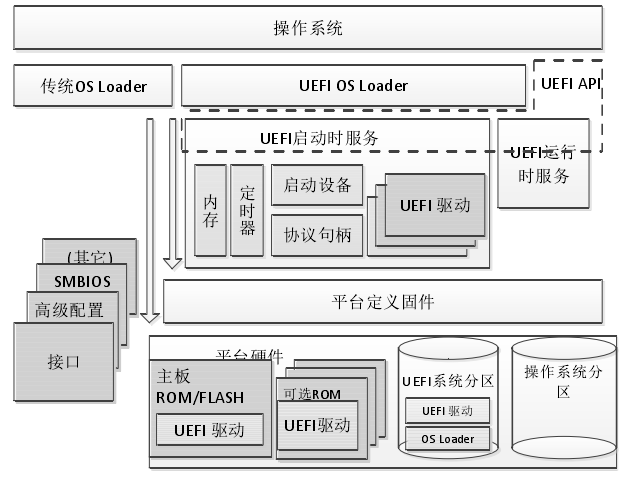
\includegraphics[width=12cm]{infrastructure_of_uefi.png}
    % 中文标题 %
    \caption*{图 2-1 UEFI系统框架图}
    % 调整图片英文标题与下文距离 %
    \setlength{\belowcaptionskip}{-0.7cm}
    % 英文标题 %
    \caption*{Figure 2-1 Infrastructure of UEFI}
\end{figure}

\par 图 2-1 描绘了UEFI框架中各模块的关系,UEFI固件作为承上启下的模块,对底层硬件进行了抽象处理,
又不断地对上层的操作系统提供服务,并在不同的服务层的连接中采用了标准的接口。图中UEFI保留了对
传统BIOS引导操作系统的兼容性,所以在可扩展固件接口的实现中有两种操作系统引导方式,分别为
Legacy OS Loader 和UEFI OS Loader。 
\par UEFI允许操作系统预处理,实现了操作系统的引导和一些系统软件执行所需要的其它应用程序,
如诊断程序、UEFI Shell、系统调试软件等,这些程序统称为UEFI实体(UEFI Image)。根据UEFI规范,
UEFI Image包含三种:UEFI应用程序、UEFI驱动和OS Loaders,这些实体都是在UEFI API调用的基础上
实现的。
\par 从图中可以看出,UEFI的启动时服务Boot Service中包含了UEFI在PEI和DXE两个主要加载驱动完成
系统初始化过程中所需要的驱动程序、内存管理、设备管理、协议贮存等信息。而UEFI的启动时服务也有他
自己的生命周期,从下图就可以看出启动时服务在UEFI启动过程中的位置。

\begin{figure}[htb]
    \label{bootint_sequence}
    % 调整图片与上文的垂直距离 %
    \vspace{0cm}   
    % 调整图片图片与中文标题、中文标题与英文标题距离 %                             
    \setlength{\abovecaptionskip}{0.3cm}  
    % 引用/fig/目录中的图片文件 %
	\centering
    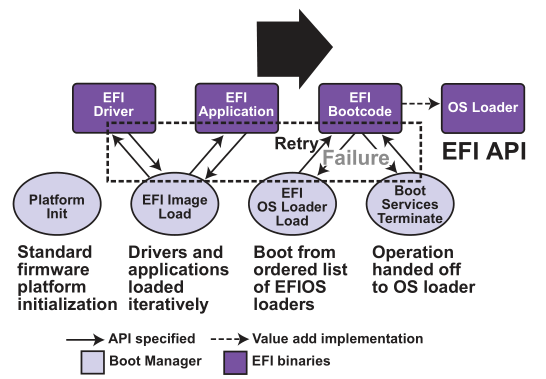
\includegraphics[width=10cm]{boot_seq.png}
    % 中文标题 %
    \caption*{图 2-2 UEFI启动流程图}
    % 调整图片英文标题与下文距离 %
    \setlength{\belowcaptionskip}{-0.7cm}
    % 英文标题 %
    \caption*{Figure 2-2 Booting Sequence of UEFI}
\end{figure}

从图2-2中可以看出,Platform Init平台初始化过程中建立Boot Service系统服务和RunTime Service系统服务,
EFI Image Load阶段包括了
PEI和DXE两个主要驱动加载过程,负责加载BIOS固件中的UEFI驱动和UEFI应用程序的EFI可执行文件,之后在启动
设备选择也就是BDS阶段中,通过用户的选择,UEFI BIOS选择适当的操作系统引导程序进行加载,并同时退出
Boot Service服务,并继续向上层操作系统提供RunTime Service服务。因而在操作系统运行过程中,可以继续使
用底层UEFI BIOS提
供的运行时服务。结合图2-1也可以发现,UEFI的一些关键驱动程序,和OS Loader也会存放在如硬盘块设备的ESP
(EFI System Partition)系统分区中。由于本文主要对于UEFI启动过程中的DXE、BDS阶段进行安全方案设计,
因此,启动时服务其中包含的如协议加载函数等为本文的主要研究对象。

\subsection{UEFI协议运作方式}
UEFI中协议设计的思想为,由于UEFI的官方提供实现的版本为C语言实现,而C语言是一种面向过程的语言,而完全
使用面向过程的思想来管理和使用众多UEFI协议将会使程序变得非常复杂。Protocol作为一种对象来设计管理会更加
直观。因而UEFI中的Protocol引入了面向对象的思想,其中包括:
\begin{itemize}
\item 用struct来模拟class。
\item 用函数指针(Protocol的成员变量)模拟成员函数,此种函数的第一参数必须是指向Protocol的指针,用来
模拟this指针。
\end{itemize}
\par 从图2-1中可以看出,UEFI中的协议包含于UEFI启动时服务中(Boot Services),由启动时服务提供的功能进行
协议的加载、保存和调用等操作。其中UEFI启动时服务提供的协议相关的功能函数如表2-1所示。

\begin{table}[htb]
    \label{tab:parametervalues}
    % 设置表内行间距 %
    \renewcommand\arraystretch{1.5}
    % 设置表题目 %
	\caption*{表 2-1 启动时服务协议功能表}
	\caption*{Table 2-1 Boot Service Protocol Interface Functions}
    \begin{tabular*}{\hsize}{@{}@{\extracolsep{\fill}}ccl@{}}
    % 表上线和表头 %
	\toprule[0.75pt]
    名称  &类型  &\makecell[c]{描述}\\
    % 表中线和表内容 %
	\midrule[0.5pt]
	InstallProtocolInterface   &Boot  &\quad 在设备句柄上安装一个协议接口\\
    UninstallProtocolInterface &Boot  &\quad 从设备句柄上移除一个协议接口\\
    ReinstallProtocolInterface &Boot  &\quad 在设备句柄上重新安装协议接口\\
    RegisterProtocolNotify     &Boot  &\makecell[l]{ 
                                       \quad 注册一个事件,只要接口有信号为指定的\\
                                             协议安装\\
                                        }\\
    LocateHandle               &Boot  &\quad 返回支持指定协议的句柄数组\\
    HandleProtocol             &Boot  &\quad 查询句柄以确定它是否支持指定的协议\\
    LocateDevicePath           &Boot  &\makecell[l]{
                                       \quad 找到支持指定路径的设备路径上的所有设\\
                                             备协议并将句柄返回到最接近的设备路径
                                        }\\
    OpenProtocol               &Boot  &\quad 将元素添加到使用协议的代理列表中接口\\
    CloseProtocol              &Boot  &\makecell[l]{
                                       \quad 从代理列表中移除一个元素,也就是消耗\\
                                             一个协议接口
                                        }\\
    OpenProtocolInformation    &Boot  &\quad 检索当前正在使用的代理列表协议接口\\
    ConnectController          &Boot  &\makecell[l]{
                                       \quad 使用一组优先规则来找到最佳的驱动程序\\
                                             集管理一个控制器
                                        }\\
    DisconnectController       &Boot  &\quad 通知一组驱动程序以停止管理控制器\\
    ProtocolsPerHandle         &Boot  &\makecell[l]{
                                       \quad 检索安装在句柄上的协议列表,函数返回\\
                                             的缓冲区是自动分配的
                                        }\\
    LocateHandleBuffer         &Boot  &\makecell[l]{
                                       \quad 从句柄数据库中检索句柄列表,该列表符\\
                                             合搜索条件,返回缓冲区自动已分配
                                        }\\
    LocateProtocol             &Boot  &\makecell[l]{
                                       \quad 在句柄数据库中找到第一个支持所需协议\\
                                             的句柄\\
                                        }\\
    InstallMultipleProtocolInterfaces
                               &Boot  &\quad 将一个或多个协议接口安装到指定句柄上\\
    UninstallMultipleProtocolInterfaces
                               &Boot  &\quad 从指定句柄中卸载一个或多个协议接口\\
    % 表下线 %
	\bottomrule[0.75pt]
    \end{tabular*}
    % 表格与下文距离 %
	\vspace{-0.3cm}
\end{table}

表2-1中列出了Boot Service中包含的所有UEFI协议相关的功能函数,其中最为常见的如InstallMultip
leProtocolInterfaces这样的加载协议函数,在众多UEFI应用以及底层驱动程序中都十分常见,因为他
可以同时提供出需要加载的多个协议GUID。
\par 同时,由于启动时服务提供了追踪最新安装了的新协议内容以及他们的使用情况,因此对于UEFI的启动时服务
来说,它可以安全地卸载并重新安装由UEFI驱动程序使用的协议接口。

\begin{figure}[htb]
    \label{bootint_sequence}
    % 调整图片与上文的垂直距离 %
    \vspace{0cm}   
    % 调整图片图片与中文标题、中文标题与英文标题距离 %                             
    \setlength{\abovecaptionskip}{0.3cm}  
    % 引用/fig/目录中的图片文件 %
	\centering
    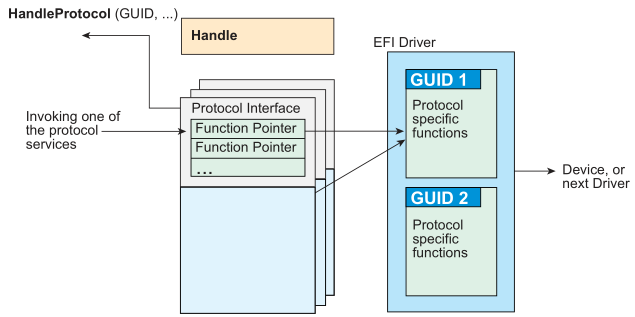
\includegraphics[width=10cm]{locate_protocol.png}
    % 中文标题 %
    \caption*{图 2-3 UEFI协议加载方式图}
    % 调整图片英文标题与下文距离 %
    \setlength{\belowcaptionskip}{-0.7cm}
    % 英文标题 %
    \caption*{Figure 2-3 Locating Protocol of UEFI}
\end{figure}

\par 协议的加载过程可通过图2-3分析得知。在图2-3中可以看出,协议由HandleProtocol等表2-1中列出的装载协议
用的功能函数加载到Handle句柄上,而所有的Handle则由UEFI内核统一存储于句柄数据库,句柄数据库也是一个链表
结构用于存储记录所有的Handle句柄,这些句柄可由任意的UEFI Image(镜像)访问,从而达到函数调用的效果。而这
些协议中包含的是指向具体函数的C语言中的函数指针,这些具体函数则是在DXE阶段由UEFI系统表提供的加载驱动镜像函数
加载并驻留在内存中的。

%
% 2.2节
%
\section{UEFI固件文件系统数据存储方式介绍}
UEFI固件文件系统指的是BIOS闪存芯片中的数据存储格式,它通过统一的固件文件系统标准用来统一闪存芯片中的文件
内容和UEFI启动阶段内存中文件的内容。具体的固件中UEFI可执行程序文件存储格式如图2-4所示。

\begin{figure}[htb]
    \label{ffs_format}
    % 调整图片与上文的垂直距离 %
    \vspace{0cm}   
    % 调整图片图片与中文标题、中文标题与英文标题距离 %                             
    \setlength{\abovecaptionskip}{0.3cm}  
    % 引用/fig/目录中的图片文件 %
	\centering
    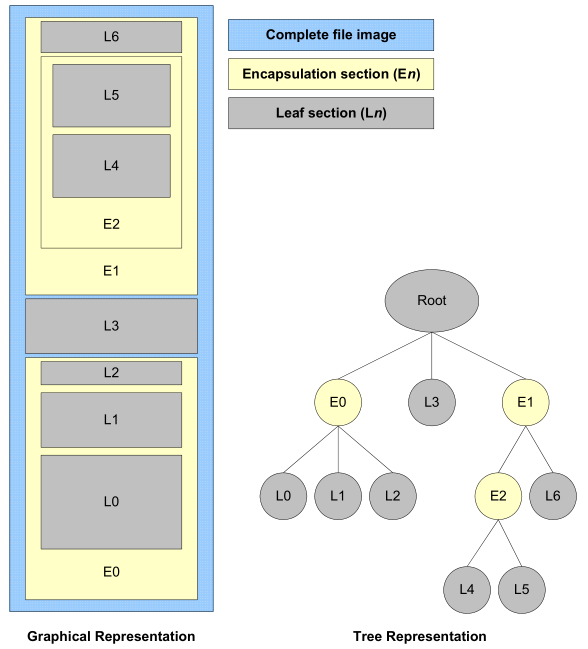
\includegraphics[width=10cm]{ffs_struct.PNG}
    % 中文标题 %
    \caption*{图 2-4 固件文件系统文件存储格式}
    % 调整图片英文标题与下文距离 %
    \setlength{\belowcaptionskip}{-0.7cm}
    % 英文标题 %
    \caption*{Figure 2-4 Firmware file system file storage format}
\end{figure}

在图2-4中,左边为通过结构图的方式说明固件文件系统的数据存储格式,右边为通过数据结构中的树形结构来阐述
FFS中的文件存储。右图中,蓝色方框代表了一个完整的FFS中的文件映像也就是UEFI中可执行文件的二进制数据,
黄色方框代表了一个父目录结构,黄色方框中包含的灰色方框代表了父目录中的子目录,也就是文件影响中的最小
单位。对应到右图的树结构中,黄色节点就是树中有子节点的父节点,而灰色节点则代表了叶子节点。了解固件文件
系统中的文件数据存储格式有助于理解UEFI内核在系统初始化过程中调用相关解析FFS中文件函数的运行过程,也有
助于帮助分析本文安全方案中可信度量的具体数据内容。
%
% 2.3节
%
\section{UEFI文件系统协议栈}

\subsection{总体介绍}

\subsection{相关驱动介绍}

%
% 2.4节
%
\section{BMC技术介绍}

\subsection{BMC在系统中的位置}

\subsection{BMC与BIOS通讯方式}

%
% 2.5节
%
\section{可信计算技术}

\subsection{可信计算信任链}

\subsection{可信平台模块}

